\section*{Question 2}
On veut à présent montrer que la suite des polynômes :
$$
\begin{array}{ccc}
f_0(x) & = & p_n(x)\\
f_1(x) & = & p_{n-1}(x)\\
&\vdots &\\
f_n(x) & = & p_0(x)
\end{array}
$$
forme une suite de Sturn sur $] - \infty, +\infty]$. Une suite de Sturn est caractérisée par quatre propriétés essentielles :

\begin{enumerate}
  \item $f_0(\alpha) f_0(\beta) \neq 0$;
  \item $f_i( \xi)=0$ avec $i \geq 1$, $\xi \in (\alpha, \beta)$, alors $f_{i-1}( \xi) f{i+1}( \xi) <0$;
  \item $f_0( \xi )=0 $ avec $\xi \in (\alpha, \beta)$, alors $f_0'( \xi ) f_1( \xi ) >0$;
  \item $f_0$ est constant sur $] \alpha, \beta]$
\end{enumerate}

Montrons que la suite des polynômes satisfait bien à ces quatre propriétés.
Pour cela, commençons par montrer que $p_n$ est un polynôme de degré $n$
et que le coefficient de $x_n$ est 1.
Cela peut être montré par induction à l'aide de l'équation de récurrence
\eqref{equ_recur}.

\begin{itemize}
  \item C'est évident pour $p_0(x)$ qui vaut 1.
  \item Si $p_{n-1}(x)$ est de degré $n-1$ et $p_{n-2}(x)$ est de degré
    $n-2$, $p_n(x)$ qui vaut
    \[ p_n(x) = xp_{n-1}(x) - (\alpha_np_{n-1}(x) + \beta_n^2p_{n-2}(x)) \]
    est la somme entre un polynôme de degré $n$ et un polynôme de
    degré au plus $n-1$ ce qui fait un polynôme de degré $n$.
    Il n'y aura qu'un terme en $x^n$ dans le terme $xp_{n-1}(x)$ donc
    le coefficient devant $x^n$ sera le même que celui devant $x^{n-1}$ qui,
    par l'hypothèse de récurrence, vaut 1.
\end{itemize}


À présent, remarquons à l'aide de l'équation de récurrence \eqref{equ_recur}
que si $(x-x_0)$ divise $p_n$ et $p_{n-1}$, alors il divise
$p_{n-2}$; et que s'il divise $p_{n-1}$ et $p_{n-2}$, alors il divise $p_n$.
On conclut que $\pgcd(p_n, p_{n-1}) = \pgcd(p_{n-1}, p_{n-2})$.


Comme $p_0(x) = 1$, $\pgcd(p_1,p_0) = p_0$ et donc, par transitivité,
$\pgcd(p_n, p_{n-1}) = p_0 = 1$.
Dès lors, on sait que $p_n$ et $p_{n-1}$ n'ont pas de racine commune.


On remarque que la matrice obtenue en supprimant
la dernière ligne et la dernière colonne de $T_n$ est par définition $T_{n-1}$.
Par le théorème 1, on sait que leurs valeurs propres sont entrelacées.
Comme leurs valeurs propres sont les racines des polynômes $p_n$ et $p_{n-1}$, on peut dire que leurs racines sont entrelacées.

Dès lors, si $p_i$ a une racine multiple $r$, $p_{i+1}$ et $p_{i-1}$
(s'ils existent) ont nécessairement cette racine.
En effet, il existera un $k$ tel que
$\lambda_k = \lambda_{k+1} = r$ et donc $\mu_{k} = r$.
Or on sait que $p_i$ et $p_{i+1}$ n'ont pas de racines communes;
de même pour $p_i$ et $p_{i-1}$.
On conclut que $p_i$ n'a pas de racines multiples.


	Nous pouvons à présent montrer que notre suite $p_i$ est une suite de Sturn.
\begin{enumerate}
  \item Commençons par montrer que $f_0(\alpha)f_0(\beta) \neq 0$.
    Comme $\alpha = -\infty$ et $\beta = + \infty$ et que $f_0$ est un polynôme,
    il faudrait que $f_0$ soit le polynôme nul.
    Pourtant, on a montré que $p_n$ est de degré $n$ et $p_0 = 1$ donc
    c'est impossible.
  \item Montrons ensuite que si $f_i(\xi) = 0$ avec $1 \leq i \leq n-1$,
    alors $f_{i-1}(\xi)f_{i+1}(\xi) < 0$.
    On peut réécrire l'équation de récurrence \ref{equ_recur} en $x=\xi$.
    Et comme par hypothèse, $f_i(\xi)=0$, on obtient la relation
    $f_{i+1}(\xi) = -\beta_n^2f_{i-1}(\xi)$, ce qui implique que
    \[ f_{i-1}(\xi)f_{i+1}(\xi) = -(\beta_nf_{i-1}(\xi))^2 < 0. \]
    En effet, d'une part $\beta_n \neq 0$ et d'autre part, comme montré précédemment, $f_i$ et $f_{i-1}$ ne peuvent
    pas avoir de racines communes, ce qui signifie que $f_{i-1}(\xi) \neq 0$.
  \item Montrons à présent que si $f_0(\xi) = 0$,
    alors $f_0'(\xi)f_1(\xi) > 0$.

    Commençons par montrer que si $\epsilon > 0$ est tel que
    $f_1(x) \neq 0$ $\forall x \in [\xi - \epsilon; \xi]$, alors
    $f_0(\xi-\epsilon) f_1(\xi-\epsilon) < 0$.

    \begin{proof}
      Comme les racines sont entrelacées,
      $f_1(x) \neq 0$ $\forall x \in [\xi - \epsilon; \xi]$ implique que
      $f_0(x) \neq 0$ $\forall x \in [\xi - \epsilon; \xi[$
      et par la continuité des polynômes, le signe de $f_1$ et $f_0$ ne change pas
      sur $[\xi - \epsilon; \xi[$.
      De plus, en $-\infty$,
      le signe de $f_0$ est $(-1)^n$ car c'est un polynôme de
      degré $n$ et que le coefficient de $x^n$ est 1.
      De la même manière, celui de $f_1$ est $(-1)^{n-1}$,
      ils sont donc de signe opposé en $-\infty$ (illustration graphique à la figure \ref{figure_Tcheb}).


      À chaque fois que $f_0$ (resp. $f_1$) traverse une racine, son signe change.
      En effet, on a prouvé qu'il n'y avait que des racines simples.
      S'il ne changeait pas de signe, $f'_0$ (resp. $f'_1$) aurait
      aussi une racine en $\xi$.
      Or on sait qu'une fonction possédant une racine de multiplicité $p > 0$
      voit sa dérivée posséder cette même racine avec une multiplicité de $p-1$.
      Ici, comme $\xi$ est une racine simple de $f_0$ (resp. $f_1$),
      cela ne peut pas être une racine de $f'_0$ (resp. $f'_1$).

      Comme les racines sont entrelacées, dans l'intervalle $]-\infty; \xi[$,
      il y a le même nombre de racines de $f_0$ que de racines de $f_1$.
      Ils ont donc changé de signe le même nombre de fois.
      Ils sont dès lors toujours de signe opposé comme en $-\infty$.
    \end{proof}

    Soit $\epsilon > 0$ tel que
    $f_1(x), f_0'(x) \neq 0$ $\forall x \in [\xi - \epsilon, \xi]$.
    On sait que $f_0'(\xi)f_0(\xi - \epsilon) < 0$.
    En effet, soit $q(x)$ tel que $q(\xi) \neq 0$ et
    $f_0(x) = (x - \xi) q(x)$.
    Comme $f_0(x) \neq 0$
    $\forall x \in [\xi-\epsilon;\xi[$, on a aussi
    $q(x) \neq 0$ $\forall x \in [\xi - \epsilon;\xi]$.
    On a $f_0'(x) = q(x) + (x - \xi) q'(x)$ d'où
    $f_0(\xi - \epsilon) = -\epsilon q(\xi - \epsilon)$ et
    $f_0'(\xi) = q(\xi)$.

    La fonction $q$ est un polynôme et est par conséquent continu sur $]-\infty, +\infty[$.
    Et comme il ne possède pas de racines entre $\xi - \epsilon$ et $\xi$,
    $q(\xi - \epsilon)$ et $q(\xi)$ sont de même signe.
    Avec le même raisonnement on montre que $f_1(\xi - \epsilon)$ et
    $f_1(\xi)$ sont de même signe.
    Comme $\epsilon > 0$, on peut déduire que $p_0'(\xi)$ et
    $p_0(\xi - \epsilon)$ sont de signe opposé.
    Puisqu'on sait que $p_0(\xi - \epsilon)$ et $p_1(\xi - \epsilon)$ sont
    de signe opposé, on obtient finalement $p_0'(\xi) p_1(\xi) > 0$.
  \item Le fait que $f_n(x)$ soit de signe constant est trivial car
    $f_n(x) = p_0(x) = 1$.
\end{enumerate}

\begin{figure}
  \centering
  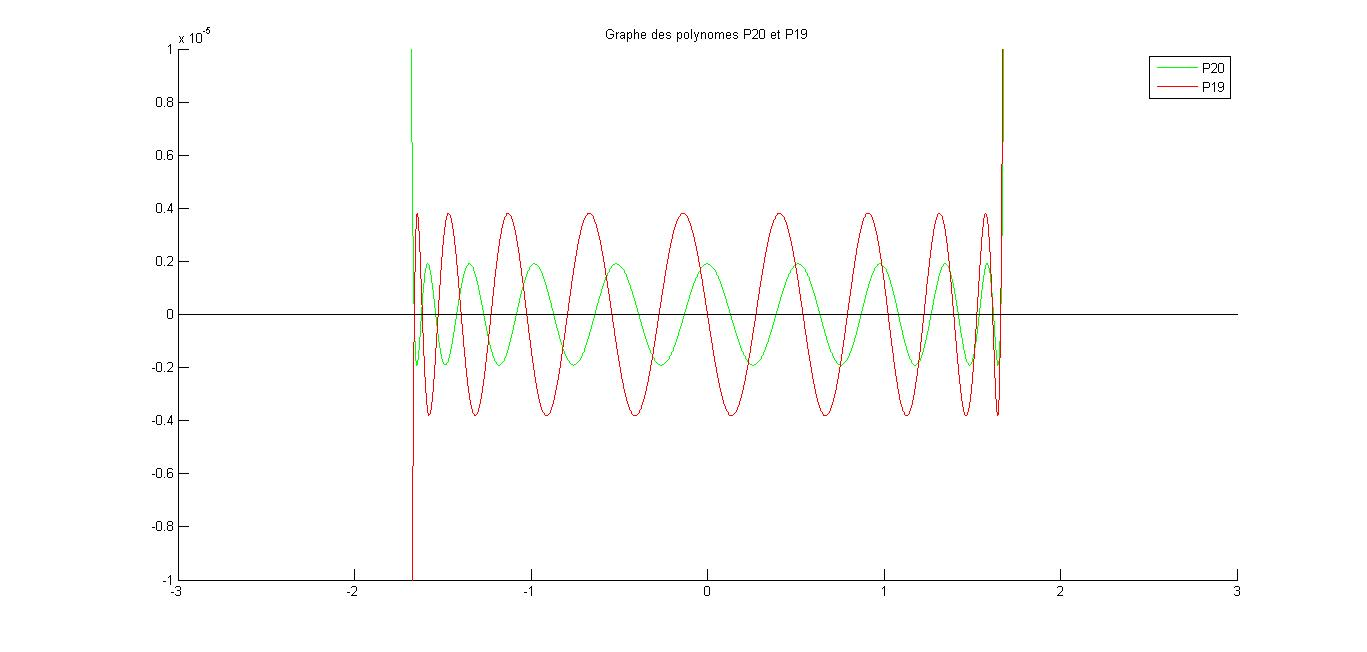
\includegraphics[height=8cm]{fig3.jpg}
  \caption{Pour illustrer la suite des polynômes $P_i$,
  nous avons tracé le graphe des polynômes $P_{20}(x)$ et $P_{19}(x)$ de
  Tchebychev (cf. Question 4).
  On remarque que les deux fonctions sont bien entrelacées.
  On voit également que le polynôme $P_{20}(x)$ a bel et bien deux racines dans
  l'intervalle $[1/2, 3/4]$,
  ce qui confirme les résultats obtenus à la question 4.}
  \label{figure_Tcheb}
\end{figure}
